\documentclass[11pt, a4paper]{article}

\usepackage{amsmath}
\usepackage{amssymb}
\usepackage{array}
\usepackage{longtable}
\usepackage{multirow}
\usepackage{listings}
\usepackage{xcolor}
\usepackage{siunitx}
\usepackage{seqsplit}
\usepackage{kotex}
\usepackage{booktabs}
\usepackage{caption}
\usepackage{tabularx}

\usepackage{makecell}


\usepackage{fontspec}
\setmainfont{Noto Serif CJK KR}

\usepackage{graphicx}
\usepackage{geometry}
\geometry{margin=0.5in}

\usepackage{hyperref}
\hypersetup{
    colorlinks=true,
    linkcolor=blue,
    urlcolor=blue,
    citecolor=blue
}

\usepackage{float}

\title{MIMIC 기반 기존 연구 리뷰 및 재현 보고서 \\ Appendix}
\author{2024404060 강민혁}
\date{}

\begin{document}

\maketitle

\section{기흉이란}


\begin{figure}[htbp]
  \centering
  \includegraphics[width=1.0\textwidth]{figures/chest_pa_with_visualization.png}
  \caption{Pneumothorax X-ray with Visualization}
  \label{fig:chest_pa_with_visualization}
\end{figure}


폐에 여러 원인으로 구멍이 생겨 새어나온 공기가 흉강에 차서, 폐를 압박해 찌그러뜨리는 질환이며, 외상성 기흉은 외부의 물리적 충격으로 인해 폐나 흉벽이 손상되어 발생하는 기흉이다.


\section{소프트웨어 환경 및 버전}

\begin{table}[htbp]
  \centering
  \caption{Environment and Key Library Versions}
  \label{tab:environment}
  \renewcommand{\arraystretch}{1.1}
  \begin{tabular}{lc}
    \toprule
    \textbf{Software / Library} & \textbf{Version} \\
    \midrule
    Python & 3.12.12 \\
    CUDA & 13.0 \\
    \midrule
    Pandas & 2.3.3 \\
    NumPy & 2.3.4 \\
    SciPy & 1.16.3 \\
    Matplotlib & 3.10.8 \\
    Seaborn & 0.13.2 \\
    Statsmodels & 0.14.5 \\
    Scikit-learn & 1.7.2 \\
    XGBoost & 3.1.2 \\
    SHAP & 0.48.0 \\
    \bottomrule
  \end{tabular}
\end{table}

\section{수식 정의}

\subsection{산소화 지수 (Oxygenation Index)}
주요 예측 인자인 Oxygenation Index의 산출 공식은 다음과 같다.
\begin{equation}
    \text{Oxygenation Index} = \frac{\text{FiO}_2 \times \text{MAP}}{\text{PaO}_2} \times 100
    \label{eq:oi}
\end{equation}

\subsection{복합 목적 함수 (Composite Objective Function)}
하이퍼파라미터 최적화를 위해 AUROC에 재현율 가중치를 결합한 목적 함수를 다음과 같이 구성하였다.
\begin{equation}
    \text{Score} = \text{AUROC} + \alpha \times \text{Recall}
    \label{eq:composite_objective}
\end{equation}

\subsection{제약 조건 기반 임계값 최적화}
모델의 최종 예측 단계에서 임상적 안전성을 보장하기 위한 제약 조건은 다음과 같다.
\begin{equation}
    \text{Recall}(t) \ge 0.45 \label{eq:recall_constraint}
\end{equation}
\begin{equation}
    \text{Accuracy}(t) \ge 0.85 \label{eq:accuracy_constraint}
\end{equation}

\section{예측 모델에 사용된 변수 정의}

\begin{table}[htbp]
  \centering
  \small
  \caption{Definitions of the 12 Key Variables Selected for the Predictive Model}
  \vspace{-0.5em}
  \label{tab:selected_variables}
  \renewcommand{\arraystretch}{1.2}
  \begin{tabularx}{\textwidth}{l l X}
    \toprule
    \textbf{Variable} & \textbf{Unit} & \textbf{Description} \\
    \midrule
    pH & - & Indicator of the acid-base status of the blood \\
    Hemoglobin & g/dL & Protein concentration reflecting the oxygen-carrying capacity of the blood \\
    PaO$_2$ & mmHg & Partial pressure of arterial oxygen; reflects dissolved oxygen tension \\
    Lactate & mmol/L & Marker of tissue hypoxia and anaerobic metabolism \\
    Oxygenation Index & - & Calculated index assessing the severity of respiratory failure \\
    SpO$_2$ & \% & Peripheral oxygen saturation; percentage of oxygen-bound hemoglobin \\
    Base Excess & mEq/L & Measure of metabolic acid-base status, independent of respiratory factors \\
    Heart Rate & bpm & Number of heartbeats per minute \\
    PaCO$_2$ & mmHg & Partial pressure of arterial carbon dioxide; indicator of alveolar ventilation \\
    Systolic BP & mmHg & Arterial blood pressure during ventricular contraction \\
    Diastolic BP & mmHg & Arterial blood pressure during ventricular relaxation \\
    Respiratory Rate & breaths/min & Number of breaths per minute \\
    \bottomrule
  \end{tabularx}
  \footnotesize
  \scriptsize
  \vspace{0.5em}
  \textit{Note: PaO$_2$, partial pressure of oxygen; SpO$_2$, peripheral oxygen saturation; PaCO$_2$, partial pressure of carbon dioxide; BP, blood pressure.}
\end{table}

\section{하이퍼파라미터 설정}

\subsection{베이스라인 모델}
\begin{table}[htbp]
  \centering
  \footnotesize
  \caption{Baseline Model XGBoost Hyperparameter Search Range and Optimal Values}
  \label{tab:hyperparameters_baseline}
  \renewcommand{\arraystretch}{0.8}
  \setlength{\tabcolsep}{4pt}
  \begin{tabular}{l c l l}
    \toprule
    \textbf{Hyperparameter} & \textbf{Symbol} & \textbf{Search Range} & \textbf{Optimal Value} \\
    \midrule
    Number of Estimators & $M$ & $\{100, 200, 300\}$ & 100 \\
    Max Depth & $d_{\max}$ & $\{3, 5, 7\}$ & 5 \\
    Learning Rate & $\eta$ & $\{0.01, 0.05, 0.1\}$ & 0.05 \\
    Subsample Ratio & $r_{\text{sub}}$ & $\{0.8, 1.0\}$ & 0.8 \\
    Column Subsample Ratio & $r_{\text{col}}$ & $\{0.8, 1.0\}$ & 1.0 \\
    Min Child Weight & $w_{\min}$ & $\{1, 3, 5\}$ & 1 \\
    Min Split Loss & $\gamma$ & $\{0, 0.1, 0.2\}$ & 0.2 \\
    \bottomrule
  \end{tabular}
\end{table}

\subsection{제안 모델}
\begin{table}[htbp]
  \centering
  \footnotesize
  \caption{Proposed Model XGBoost Hyperparameters via Bayesian Optimization}
  \label{tab:hyperparameters_proposed}
  \renewcommand{\arraystretch}{0.8}
  \setlength{\tabcolsep}{4pt}
  \begin{tabular}{l c l}
    \toprule
    \textbf{Hyperparameter} & \textbf{Symbol} & \textbf{Optimal Value} \\
    \midrule
    Number of Estimators & $M$ & 327 \\
    Max Depth & $d_{\max}$ & 10 \\
    Learning Rate & $\eta$ & 0.0117 \\
    Subsample Ratio & $r_{\text{sub}}$ & 0.959 \\
    Column Subsample Ratio & $r_{\text{col}}$ & 0.627 \\
    Min Child Weight & $w_{\min}$ & 2 \\
    Min Split Loss & $\gamma$ & 0.0096 \\
    L1 Regularization & $\alpha_{\text{reg}}$ & 0.0029 \\
    L2 Regularization & $\lambda_{\text{reg}}$ & $3.22 \times 10^{-8}$ \\
    \bottomrule
  \end{tabular}
\end{table}

\section{상세 실험 결과}

\subsection{제약 조건 기반 임계값 최적화 결과}
제안 모델에서 제약 조건 기반 임계값 최적화를 수행한 결과, 최적 임계값은 0.650으로 결정되었다. 이는 최소 민감도 제약($\text{Recall} \ge 0.45$)과 최소 정확도 제약($\text{Accuracy} \ge 0.85$)을 동시에 만족하면서 F1-score를 최대화하는 지점이다.

\begin{table}[H]
\centering
\footnotesize
\caption{Cross-Validation Results at Optimized Threshold (0.650)}
\label{tab:optimized_threshold}
\renewcommand{\arraystretch}{0.8}
\setlength{\tabcolsep}{4pt}
\begin{tabular}{lc}
  \toprule
  \textbf{Metric} & \textbf{Value (Mean $\pm$ Std)} \\
  \midrule
  AUROC & 0.904 $\pm$ 0.040 \\
  AUPRC & 0.704 $\pm$ 0.095 \\
  Accuracy & 0.883 $\pm$ 0.034 \\
  F1 Score & 0.668 $\pm$ 0.083 \\
  Precision & 0.650 $\pm$ 0.116 \\
  Recall & 0.700 $\pm$ 0.100 \\
  Specificity & 0.920 $\pm$ 0.038 \\
  PPV & 0.650 $\pm$ 0.116 \\
  NPV & 0.939 $\pm$ 0.019 \\
  \bottomrule
\end{tabular}
\end{table}

\subsection{베이스라인 대비 성능 개선}
\begin{table}[H]
\centering
\footnotesize
\caption{Performance Comparison: Baseline vs. Recall-Optimized Model}
\label{tab:improvement}
\renewcommand{\arraystretch}{0.8}
\setlength{\tabcolsep}{4pt}
\begin{tabular}{lccc}
  \toprule
  \textbf{Metric} & \textbf{Baseline} & \textbf{Proposed} & \textbf{Change} \\
  \midrule
  AUROC & 0.910 & 0.904 & -0.006 \\
  AUPRC & 0.764 & 0.704 & -0.060 \\
  Accuracy & 0.885 & 0.883 & -0.002 \\
  F1 Score & 0.557 & 0.668 & \textbf{+0.111} \\
  Precision & 0.779 & 0.650 & -0.129 \\
  Recall & 0.442 & 0.700 & \textbf{+0.258} \\
  \bottomrule
\end{tabular}
\end{table}

\subsection{SHAP 변수 중요도 분석}
\begin{table}[H]
\centering
\footnotesize
\caption{Top 10 Feature Importance by SHAP Values (Recall-Optimized Model)}
\label{tab:shap}
\renewcommand{\arraystretch}{0.8}
\setlength{\tabcolsep}{4pt}
\begin{tabular}{clc}
  \toprule
  \textbf{Rank} & \textbf{Feature} & \textbf{Mean |SHAP|} \\
  \midrule
  1 & Hemoglobin & 0.628 \\
  2 & MAP & 0.447 \\
  3 & PaO$_2$ & 0.404 \\
  4 & Lactate & 0.395 \\
  5 & SpO$_2$ & 0.379 \\
  6 & Oxygenation Index & 0.351 \\
  7 & FiO$_2$ & 0.350 \\
  8 & Base Excess & 0.332 \\
  9 & Systolic BP & 0.301 \\
  10 & Heart Rate & 0.242 \\
  \bottomrule
\end{tabular}
\end{table}

\section{결과 시각화}
\subsection{교차 검증 메트릭 비교}

\begin{figure}[H]
  \centering
  \includegraphics[width=0.9\textwidth]{figures/cv_metrics_comparison.png}
  \caption{Cross-Validation Metrics Comparison. Comparison of key performance metrics between baseline model and recall-optimized proposed model across 5-fold cross-validation.}
  \label{fig:cv_metrics_comparison}
\end{figure}

\subsection{SHAP 분석 결과}

\begin{figure}[H]
  \centering
  \includegraphics[width=0.8\textwidth]{figures/shap_importance.png}
  \caption{SHAP Feature Importance. Bar plot showing the mean absolute SHAP values for each feature, indicating their relative contribution to model predictions.}
  \label{fig:shap_importance}
\end{figure}

\begin{figure}[H]
  \centering
  \includegraphics[width=0.8\textwidth]{figures/shap_summary.png}
  \caption{SHAP Summary Plot. Each point represents a patient sample; the color indicates the feature value (red=high, blue=low), and the horizontal position shows the SHAP value (positive=increased risk of pneumothorax progression).}
  \label{fig:shap_summary}
\end{figure}

\subsection{임계값 분석}

\begin{figure}[H]
  \centering
  \includegraphics[width=0.9\textwidth]{figures/threshold_analysis.png}
  \caption{Threshold Analysis. Performance metrics (Accuracy, F1-Score, Precision, Recall) as a function of classification threshold. The optimal threshold (0.650) was selected to satisfy the recall constraint ($\ge 0.45$) and accuracy constraint ($\ge 0.85$) while maximizing F1-score.}
  \label{fig:threshold_analysis}
\end{figure}

\section{주요 예측 인자에 따른 영상 비교}
SHAP 분석 결과 Hemoglobin이 외상성 중증 기흉 예측에 가장 중요한 인자로 확인되었다. 이러한 결과의 임상적 타당성을 검증하기 위해 Figure~\ref{fig:chest_comparison}와 같이 실험군 내에서 헤모글로빈 수치에 따른 상위 0.5\%, 중위값(50\%), 하위 0.5\%에 해당하는 환자의 흉부 X선 영상을 비교 분석하였다.

\begin{figure}[htbp]
  \centering
  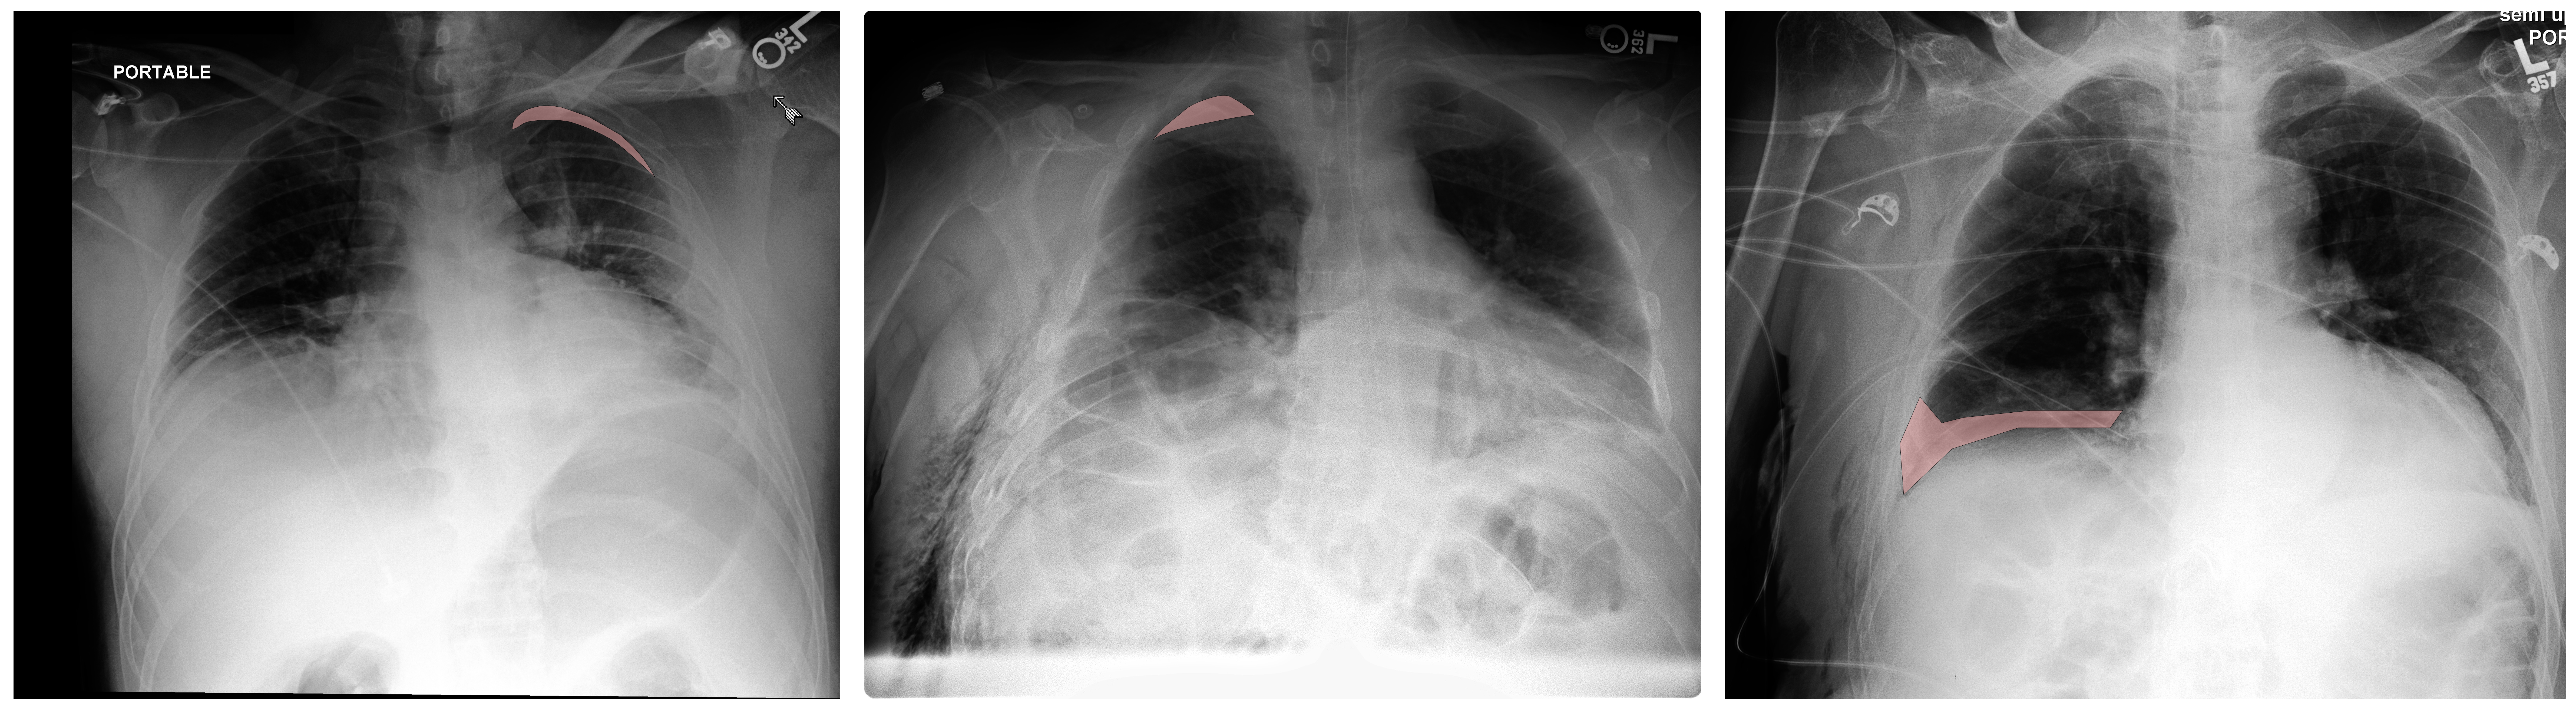
\includegraphics[width=0.8\textwidth]{figures/chest_pa_comparison.png}
  \caption{Chest X-ray Comparison by Hemoglobin Levels in Traumatic Pneumothorax Patients. Left: High hemoglobin (13.3 g/dL, top 0.5\%), Center: Median hemoglobin (10.77 g/dL), Right: Low hemoglobin (7.15 g/dL, bottom 0.5\%).}
  \label{fig:chest_comparison}
\end{figure}

\paragraph{상위 백분위수 환자 (헤모글로빈 13.3 g/dL)}
LUL상단 용적이 감소한 것을 확인할 수 있다. 동시에 cardiomegaly가 확인되며, heart failure 치료를 위한 diuretics사용으로 hemoconcentration가 일어나 헤모글로빈 수치가 상대적으로 높아진 것으로 파악된다.

\paragraph{중위 백분위수 환자 (헤모글로빈 10.77 g/dL)}
RUL상단 용적이 감수한 것을 확인할 수 있다. 우측 상복부에는 피하 기종이 파악되며, adynamic ileus가 예상된다. 헤모글로빈 수치 자체는는 임상적으로 경도의 빈혈에 해당하나, 본 데이터셋 내에서는 중위값에 해당한다. 즉, 외상성 기흉 환자군 전반에서 출혈에 따른 헤모글로빈 저하가 흔함을 확인할 수 있으며, 원인은 다양하게 나타남을 예상할 수 있다.

\paragraph{하위 백분위수 환자 (헤모글로빈 7.15 g/dL)}
multiple rib fractures 이후 산소포화도 저하와 산소 요구량 증가를 보인 환자이다. rib fractures로 인해 헤모글로빈 수치 감소가 되었음을 예상할 수 있으며, 이와같이 직접적인 외상으로 기흉, 정확히는, Hemo-pneumothorax가 발생함을 확인할 수 있었다.

\paragraph{임상적 해석} 하위 백분위수 환자의 경우, multiple rib fractures과 같은 큰손상이 동반되었으며, 이에 따른 hemothorax로 인해 헤모글로빈 수치의 급격한 저하를 유발한 것으로 판단된다. 이는 헤모글로빈 수치가 외상성 기흉의 중증도와 직결되는 출혈량 및 손상 범위를 대변한다는 점을 시사한다. 반면, 상위 백분위수 환자군에서는 cardiomegaly가 확인되며, diuretics 사용으로 인해 hemoconcentration가 일어나 수치가 높게 측정된 것으로 예상되며, 기저 질환이 있는 환자군에서의 특이적 양상으로 해석할 수 있다.

SHAP에서 헤모글로빈이 최상위 예측 인자로 도출된 것은 외상으로 인한 직접적인 출혈과 환자의 기저 상태가 중증 기흉의 예후 및 양상을 결정짓는 핵심 요인이기 때문으로 판단된다. 본 분석에서 사용된 샘플은 각 레벨에서의 하나의 Chest PA만을 가져온 것으로 일반화를 하기에는 한계가 존재하나, 헤모글로빈 수치가 외상성 기흉 환자의 중증도 분류 및 예후 예측에 있어 생리학적으로 타당한 지표임을 뒷받침할 수 있을 가능성을 시사한다.

\end{document}
